\documentclass[11pt]{article}

\usepackage{acl-hlt2011}
\usepackage{times}
\usepackage{latexsym}
\usepackage{amsmath}
\usepackage{multirow}
\usepackage{url}
\usepackage{graphicx}
\usepackage{subfig}
\usepackage{marvosym}

\setlength\titlebox{6.5cm}

\hyphenation{CachePipe}

\newcommand{\aff}{\ensuremath{{}^\text{\Radioactivity}}}
\newcommand{\afff}{\ensuremath{{}^\text{\Bat}}}
\newcommand{\grammarrule}[3]{$#1 \to \langle \text{#2} , \text{#3} \rangle$ }

\title{Joshua 3.0: Syntax-based Machine Translation with the Thrax
  Grammar Extractor}

\author{Jonathan Weese\aff, Juri Ganitkevitch\aff, Chris
  Callison-Burch\aff, Matt Post\afff \and Adam Lopez\aff\afff \\
\aff Center for Language and Speech Processing \\
\afff Human Language Technology Center of Excellence \\
Johns Hopkins University}

\date{}

\begin{document}
\maketitle

\begin{abstract}
We present progress on Joshua, an open-source decoder for hierarchical
and syntax-based machine translation.  The main focus is describing
Thrax, a flexible, open source synchronous context-free grammar
extractor.  Thrax extracts both hierarchical \cite{Chiang2007} and
syntax-augmented machine translation \cite{samt2006} grammars.  It is
built on Apache Hadoop for efficient distributed performance, and can
easily be extended with support for new grammars, feature functions,
and output formats.
\end{abstract}

\section{Introduction}

Joshua is an open-sourced toolkit for hierarchical machine translation
of human languages.  The original version of Joshua \cite{Joshua-WMT}
was a reimplementation of the Python-based Hiero machine-translation
system \cite{Chiang2007}; it was later extended \cite{li2010joshua} to
support richer formalisms, such as SAMT \cite{samt2006}.

The main focus of this paper is to describe this past year's work in
developing {\bf Thrax} \cite{jonnymasters}, an open-source grammar extractor for Hiero and
SAMT grammars.  Grammar extraction has shown itself to be something of
a black art, with decoding performance depending crucially on a
variety of features and options that are not always clearly described in papers.
This hindered direct comparison both between and within grammatical formalisms.
Thrax standardizes Joshua's grammar extraction procedures by providing
a flexible and configurable means of specifying these settings.
Section~\ref{section:results} presents a systematic comparison of the
two grammars using identical feature sets.

In addition, Joshua now includes a single parameterized script that
implements the entire MT pipeline, from data preparation to
evaluation.  This script is built on top of a module called
\emph{CachePipe}.  CachePipe is a simple wrapper around shell commands
that uses SHA-1 hashes and explicitly-provided lists of dependencies
to determine whether a command needs to be run, saving time both in
running and debugging machine translation pipelines.

\section{Thrax: grammar extraction}

In modern machine translation systems such as Joshua \cite{Joshua-WMT} and cdec \cite{cdec}, a translation model is often represented as a synchronous context-free grammar (SCFG). Formally, an SCFG may be considered as a tuple
$$(N,S,T_\sigma,T_\tau,G)$$
where $N$ is a set of nonterminal symbols of the grammar, $S \in N$ is the goal symbol, $T_\sigma$ and $T_\tau$ are the source- and target-side terminal symbol vocabularies, respectively, and $G$ is a set of {\em production rules} of the grammar.

Each rule in $G$ is of the form
$$X \to \langle \alpha , \gamma , \sim \rangle$$
where $X \in N$ is a nonterminal symbol, $\alpha$ is a (possibly mixed) sequence of symbols from $N \cup T_\sigma$, $\gamma$ is a (again, possibly mixed) sequence of symbols from $N \cup T_\tau$, and $\sim$ is a one-to-one correspondence between the nonterminal symbols of $\alpha$ and $\gamma$.

The language of an SCFG is a set of ordered pairs of strings. During
decoding, the set of candidate translations of an input sentence $f$
is the set of all $e$ such that the pair $(f,e)$ is licensed by the
translation model SCFG.  Each candidate $e$ is generated by applying a
sequence of production rules $(r_1 \ldots r_n)$.  The cost of applying each rule is:
\begin{equation}
w(X \to \langle \alpha, \gamma \rangle) = \prod_i{\phi_i(X \to \langle \alpha , \gamma \rangle)^{\lambda_i}}
\end{equation}
where each $\phi_i$ is a {\em feature function} and $\lambda_i$ is the weight for $\phi_i$.
We define the total {\em translation model score} of candidate $e$ as
\begin{equation}
w_{TM}(e) = \prod_{i=1}^n{w(r_i)}
\end{equation}

\noindent This translation model score is combined with
other features to produce an overall score for each candidate translation.

\subsection{Hiero and SAMT}

\begin{table*}[t]
  \centering
  \begin{tabular}{ccc}
    Span & Hiero & SAMT \\
\hline\hline
$[1,3]$ & \grammarrule{X}{sehr}{very much} & \grammarrule{ADVP}{sehr}{very much} \\
$[0,3]$ & \grammarrule{X}{$X$ sehr}{$X$ very much} & \grammarrule{PRP+ADVP}{$PRP$ sehr}{$PRP$ very much} \\
$[3,4]$ & \grammarrule{X}{begr\"{u}\ss{}e}{welcome} & \grammarrule{VBP}{begr\"{u}\ss{}e}{welcome} \\
$[0,6]$ & \grammarrule{X}{$X$ ich sehr .}{i very much $X$ .} & \grammarrule{S}{$VP$ ich sehr .}{i very much $VP$ .} \\
$[0,6]$ & \grammarrule{X}{$X$ .}{$X$ .} & \grammarrule{S}{$S/.$ .}{$S/.$ .} \\
  \end{tabular}
  \caption{A subset of the Hiero and SAMT rules extracted from the sentence
    pair of Figure~\ref{figure:alignment}.}
  \label{table:rules}
\end{table*}

Throughout this work, we will reference two particular SCFG types known as Hiero and Syntax-Augmented Machine Translation (SAMT).

A Hiero grammar \cite{Chiang2007} is an SCFG with only one type of
nonterminal symbol (traditionally labelled $X$).  A Hiero grammar can
be extracted from a parallel corpus where each sentence pair has been
word-aligned.  If $(f_i^j,e_k^l)$ is a sub-phrase of the sentence
pair, we say it is {\em consistent} with the pair's alignment if none
of the words in $f_i^j$ are aligned to words outside of $e_k^l$, and
vice-versa. The consistent sub-phrase may be extracted as an SCFG
rule.  Furthermore, if a consistent phrase is contained within another
one, a hierarchical rule may be extracted by replacing the smaller
piece with a nonterminal.

\begin{figure}[ht]
  \centering
  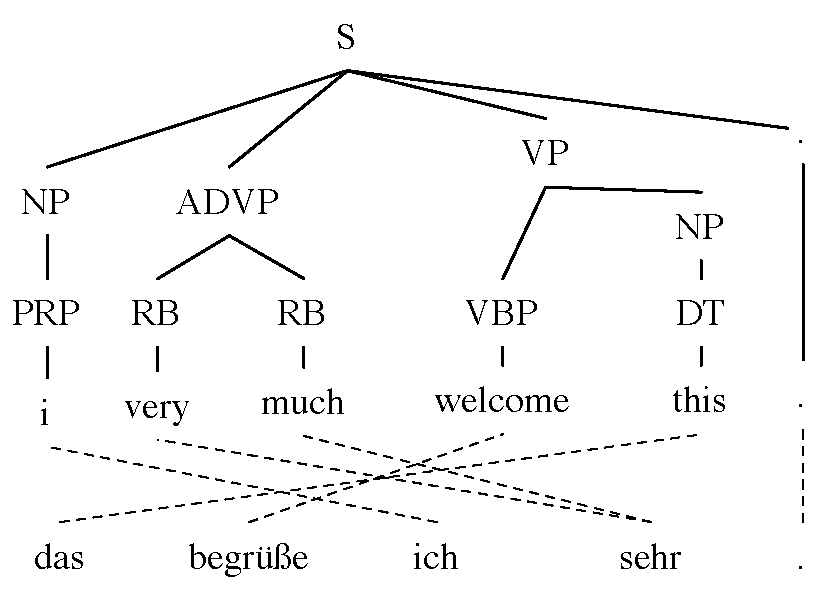
\includegraphics[width=0.4\textwidth]{figures/alignment}
  \caption{An aligned sentence pair.}
  \label{figure:alignment}
\end{figure}

An SAMT grammar \cite{samt2006} is similar to a Hiero grammar, except
that the nonterminal symbol set is much larger, and its labels are
syntactically motivated.  SAMT rules are extracted from aligned sentence pairs, but they require some additional information: they require a parse tree for the target-side sentence.

When a rule is extracted as a consistent phrase pair (as in Hiero), if
the target side is spanned by one constituent of the parse tree, we
assign that constituent's label as the nonterminal symbol for the
rule.  Otherwise, we assign an extended category of the form
$C_1+C_2$, $C_1 / C_2$, or $C_2$ \textbackslash $C_1$ --- indicating
that the target side spans two adjacent constituents, is a $C_1$
missing a $C_2$ to the right, or is a $C_1$ missing a $C_2$ on the
left, respectively.  These extended categories are adapted from
combinatory categorial grammars \cite{Steedman1999}.
Table~\ref{table:rules} contains a list of Hiero and SAMT rule
extracted from the training sentence pair in Figure~\ref{figure:alignment}.

\subsection{Related work}

We are not aware of any stand-alone grammar extraction programs. Other grammar extractors are developed and distributed with a particular MT system. We give an overview of a few such extractors here.

Joshua includes a simple Hiero extractor \cite{schwartz2010}. The extractor runs as a single Java process. This makes it difficult to extract larger grammars, as the host machine must have enough memory to hold all of the rules at once. Joshua's extractor scores each rule with three feature functions --- lexical probabilities in two directions, and one phrasal probability score $p(\gamma|\alpha)$.

The SAMT implementation of Zollmann and Venugopal \shortcite{samt2006} includes a several-thousand-line Perl script to extract their rules. In addition to phrasal and lexical probabilities, this extractor implements several other features that are also described in section \ref{features}.

Finally, the cdec decoder \cite {cdec} includes a grammar extractor that performs well only when all rules can be held in memory.

Memory usage is a serious limitation of both Joshua and cdec extractors. Translation models can be very large, and many feature scores require accumulation of statistical data from the entire set of extracted rules. Since it is impractical to keep the entire grammar in memory, rules are usually sorted on disk and then read sequentially.

Different feature calculations may require different sort orders, leading to a linear workflow that alternates between sorting the grammar and calculating a feature score. To calculate more feature scores, more sorts have to be performed. This discourages the implementation of new features. For example, Joshua's built-in rule extractor calculates the phrasal probability $p(\gamma|\alpha)$ for each rule but, to save time, does not calculate its obvious counterpart $p(\alpha|\gamma)$, which would require another sort.

The SAMT extractor does not have a problem with large data sets; SAMT
has been extended \cite{venugopal2009hadoop} to run on Hadoop, an
implementation of Google's MapReduce framework for efficient
processing of large amounts of data.  We will discuss Hadoop more in
section \ref{design}.

None of these three extractors are designed for flexibility in terms of grammar extraction. The Joshua and cdec extractors only extract Hiero grammars, and Zollmann and Venugopal's extractor can only extract SAMT-style grammars. They are not designed to score arbitrary feature sets, either.

Since variation in translation models and feature sets can have a significant effect on translation performance, we have developed Thrax in order to make it easy to build and test new models. 

\subsection{System overview}
\label{design}

The following were goals in the design of Thrax:

\begin{itemize}
\item ability to extract different SCFGs (such as Hiero and SAMT), and to adjust various extraction parameters for the grammars;
\item ability to easily change the feature set with which to score the extracted rules, and easily implement new features;
\item scalability to arbitrarily large training corpora.
\end{itemize}

Thrax treats the grammar extraction and scoring as a series of dependent Hadoop jobs. Hadoop is an implementation of Google's MapReduce \cite{mapreduce}, a framework for distributed processing of large data sets. Hadoop jobs have two parts. In the {\em map} step, a set of key/value pairs is mapped to a set of intermediate key/value pairs. In the {\em reduce} step, all intermediate values associated with an intermediate key are merged.

The first step in the Thrax pipeline is to extract all the grammar rules. The map step in this job takes as input word-aligned sentence pairs and produces a set of ordered pairs $(r,c)$ where $r$ is a rule and $c$ is the number of times it was extracted. During the reduce step, these rule counts are summed, so the result is a set of rules, along with the total number of times each rule was extracted from the entire corpus.

Given the rules and their counts, a separate Hadoop job is run for each feature. These jobs can all be submitted at once and run in parallel, avoiding the linear sort-and-score workflow. The output from each feature job is the same set of pairs $(r,c)$ as the input, except each rule $r$ has been annotated with some feature score $f$.

After the feature jobs have been completed, we have several copies of
the grammar, each of which has been scored with one feature.  A final Hadoop job combines all these scores to produce the final grammar.

Some users may not have access to a Hadoop cluster. Thrax can be run in standalone or pseudo-distributed mode on a single machine. It can also be used with Amazon Elastic MapReduce,\footnote{\url{http://aws.amazon.com/elasticmapreduce/}} a web service that provides computation time on a Hadoop cluster on-demand.

\subsection{Extraction}

The first step in the Thrax workflow is the extraction of grammar rules from an input corpus. As mentioned above, Hiero and SAMT grammars both require a parallel corpus with word-level alignments. SAMT additionally requires that the target side of the corpus be parsed.

There are several parameters that can make a significant difference in a grammar's overall translation performance. Each of these parameters is easily adjustable in Thrax by changing its value in a configuration file.

\begin{itemize}
\item maximum rule span
\item maximum span of consistent phrase pairs
\item maximum number of nonterminals
\item minimum number of aligned terminals in rule
\item whether to allow adjacent nonterminals on source side
\item whether to allow unaligned words at the edges of consistent phrase pairs
\end{itemize}

Chiang \shortcite{Chiang2007} gives reasonable heuristic choices for these parameters when extracting a Hiero grammar, and Lopez \shortcite{lopez-2008} confirms some of them (maximum rule span of 10, maximum number of source-side symbols at 5, and maximum number of nonterminals at 2 per rule). No similar parameter analysis has been performed for SAMT.

When extracting Hiero- or SAMT-style grammars, the first Hadoop job in the Thrax workflow takes in a parallel corpus and produces a set of rules. But in fact Thrax's extraction mechanism is more general than that; all it requires is a function that maps a string to a set of rules. This makes it easy to implement new grammars and extract them using Thrax.

\subsection{Feature functions}
\label{features}

Thrax considers feature functions of two types: first, there are features that can be calculated by looking at each rule in isolation. Such features do not require a Hadoop job to calculate their scores, since we may inspect the rules in any order. (In practice, we calculate the scores at the very last moment before outputting the final grammar.) We call these features {\em simple features}. Thrax implements the following simple features:
\begin{itemize}
\item a binary indicator function if the rule is purely abstract (with no terminal symbols);
\item an indicator function if the rule is purely lexical (with no nonterminals);
\item an indicator function if the rule is monotonic or has reordering;
\item an indicator function if the rule has adjacent nonterminals on the source side;
\item a counter giving the number of unaligned words in the rule;
\item a counter giving the number of terminals on the target side of the rule;
\item a constant phrase penalty.
\end{itemize}
In addition to simple features, Thrax also implements {\em map-reduce features}. These are features that require comparing rules in a certain order. Thrax uses Hadoop to sort the rules efficiently and calculate these feature functions. Thrax implements the following map-reduce features:
\begin{itemize}
\item Phrasal translation probabilities $p(\alpha|\gamma)$ and
  $p(\gamma|\alpha)$, calculated with relative frequency:
\begin{equation}
p(\alpha|\gamma) = \frac{C(\alpha,\gamma)}{C(\gamma)}
\end{equation}
(and vice versa), where $C(\cdot)$ is the number of times a given
event was extracted.
\item Lexical weighting $p_{\textit{lex}}(\alpha|\gamma,A)$ and $p_{\textit{lex}}(\gamma|\alpha,A)$. We calculate these weights as given in \cite{koehn2003}: let $A$ be the alignment between $\alpha$ and $\gamma$, so $(i,j) \in A$ if and only if the $i$th word of $\alpha$ is aligned to the $j$th word of $\gamma$. Then we can define $p_{\textit{lex}}(\gamma|\alpha)$ as
\begin{equation}
\prod_{i=1}^n{\frac{1}{|\{j : (i,j) \in A\}|}\sum_{(i,j) \in A}{w(\gamma_j|\alpha_i)}}
\end{equation}
where $\alpha_i$ is the $i$th word of $\alpha$, $\gamma_j$ is the
$j$th word of $\gamma$, and $w(y|x)$ is the relative frequency of
seeing word $y$ given $x$. 
\item Rarity penalty, given by
\begin{equation}
\exp(1 - C(X \to \langle \alpha , \gamma \rangle))
\end{equation}
where again $C(\cdot)$ is a count of the number of times the rule was extracted.
\end{itemize}

Each of the features we mentioned above can be individually included or excluded when the grammar is extracted. One can simply list the features to be included in a configuration file.

It is very easy to extend Thrax with new feature functions. For simple features, all that is needed is to implement the {\sc SimpleFeature} interface with a method that takes in a rule and calculates a feature score. Map-reduce features are slightly more complex: to subclass {\sc MapReduceFeature}, one must define a mapper and reducer, but also a sort comparator to determine in what order the rules are compared during the reduce step.


\section{Experiments}
\label{section:results}

\begin{table}
\centering
\begin{tabular}{|c|c|c|}
Language pair & sentences (K) & words (M) \\
\hline\hline
cs--en & 332 & 4.7 \\
de--en & 279 & 5.5 \\
en--cs & 487 & 6.9 \\
en--de & 359 & 7.2 \\
en--fr & 682 & 12.5 \\
fr--en & 792 & 14.4 \\
\end{tabular}
\caption{Training data size after subsampling.\label{training-data-size}}
\end{table}

We built systems for six language pairs for the WMT 2011 shared task:
cz-en, en-cz, de-en, en-de, fr-en, and en-fr.  For each language pair,
we built both SAMT and hiero grammars.\footnote{Except for fr-en and
  en-fr.  We were unable to decode with SAMT grammars for these
  language pairs due to their large size.  We have since resolved this
  issue and will have scores for the final version of the paper.}
Table~\ref{table:results} contains the results on the complete WMT
2011 test set.

To train the translation models, we used the provided Europarl and
news commentary data. For cz-en and en-cz, we also used sections of
the CzEng parallel corpus \cite{czeng:pbml:2009}.  The parallel data
was subsampled using Joshua's built-in subsampler to select sentences
with n-grams relevant to the tuning and test set.  We used SRILM to train a 5-gram language model with Kneser-Ney smoothing using the appropriate side of the parallel data. For the English LM, we also used English Gigaword Fourth Edition.\footnote{LDC2009T13}

Before extracting an SCFG with Thrax, we used the provided Perl
scripts to tokenize and normalize the data. We also removed any
sentences longer than 50 tokens (after tokenization).  For SAMT
grammar extraction, 
we parsed the English training data using the Berkeley Parser
\cite{petrov2006learning} with the
provided Treebank-trained grammar.

\begin{figure*}[t]
  \centering
  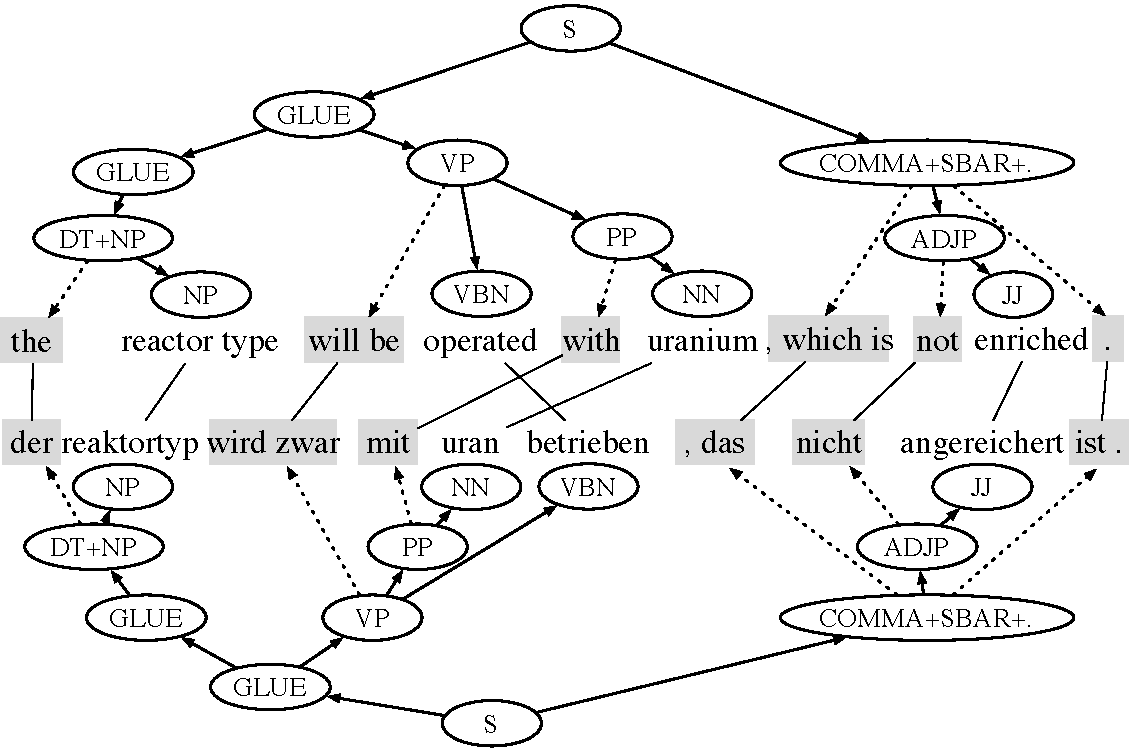
\includegraphics[width=0.8\textwidth]{figures/derivation}
  \caption{An SAMT derivation.}
  \label{figure:derivation}
\end{figure*}

We tuned the model weights against the WMT08 test set ({\tt news-test2008}) using Z-MERT \cite{zaidan2009z}, an
implementation of minimum error-rate training included with Joshua.  We decoded the test set to produce a 300-best list of unique
translations, then chose the best candidate for each sentence using
Minimum Bayes Risk reranking \cite{kumar2004minimum}.
Figure~\ref{figure:derivation} shows an example derivation with an
SAMT grammar.  To re-case the 1-best test set output, we trained a true-case language
model using the same LM training data as before.  We used an SCFG
translation model to translate from the lowercased to true-case
output.  The translation model used rules limited to five tokens in length, and contained no hierarchical rules. 

\begin{table}[t]
  \centering
  \begin{tabular}{l|rrr}
    pair   & hiero & SAMT & improvement \\
    \hline\hline
    cz-en  & 21.1  & 21.7 & +0.8 \\
    en-cz  & 16.8  & 16.9 & +0.1 \\
    de-en  & 18.9  & 19.5 & +0.6 \\
    en-de  & 14.3  & 14.9 & +0.6 \\
    fr-en  & 28.0  & - & - \\
    en-fr  & 30.4  & - & - \\
  \end{tabular}
  \caption{Single-reference BLEU-4 scores.}
  \label{table:results}
\end{table}

\section{CachePipe: Cached pipeline runs}

Machine translation pipelines involve the specification and execution
of many different datasets, training procedures, and pre- and
post-processing techniques that can have large effects on translation
outcome, and which make direct comparisons between systems difficult.
The complexity of managing these pipelines and experimental
environments has led to a number of different experimental management
systems, such as
Experiment.perl,\footnote{\url{http://www.statmt.org/moses/?n=FactoredTraining.EMS}}
Joshua 2.0's Makefile system \cite{li2010joshua}, and LoonyBin
\cite{clark2010loonybin}.  In addition to managing the pipeline, these
scripts employ different techniques to avoid expensive recomputation
by caching steps.  However, these
approaches are based on simple but unreliable heuristics (such as
timestamps or file existence) to make the
caching determination.

Our solution to the caching dependency problem is CachePipe.
CachePipe is designed with the following goals: (1) robust
content-based dependency checking, and (2) ease of use, including
minimal editing of existing scripts.  CachePipe is essentially a
wrapper around command invocations.  Presented with a command to run
and a list of file dependencies, it computes SHA-1 hashes of the
dependencies and of the command invocation and stores them; the
command is executed only if any of those hashes are different from
previous runs.  A basic invocation involves specifying (1) a name or
identifier associated with the command or step, (2) the command to
run, and (3) a list of file dependencies.  For example, to copy file
\verb|a| to \verb|b| from a shell prompt, the following command could
be used:

\verb|cachecmd copy "cp a b" a b|

\noindent The first time the command is run, the file would be copied;
afterwards, the command would be skipped after CachePipe verified that
the contents of the dependencies and had not changed.

CachePipe is open-source software, distributed with Joshua or
available
separately.\footnote{\url{https://github.com/mjpost/cachepipe}} It
currently provides both a shell script interface and a programmatic
API for Perl.  It accepts a number of other arguments and dependency
types.  It also serves as the foundation of a new script in Joshua 3.0
that implements the complete Joshua pipeline, from data preparation to
evaluation.

\section{Future work}

Thrax is currently limited to SCFG-based translation models.  A natural
development would be to extract GHKM grammars \cite{galley2004whats}
or more recent tree-to-tree models
\cite{zhang2008,liu2009,chiang2010}.  We also hope that Thrax will
continue to be extended with more feature functions as researchers
develop and contribute them.

%% \section{Acknowledgments}
%% - grants
%% - Adam Lopez for help brainstorming CachePipe

\bibliographystyle{acl}
\bibliography{thrax}

\end{document}
